%!TEX root = main.tex
\chapter{Polyphonie/Message domain}
\label{polyphonie}
\section{Notizen}

\textbf{Vor der übung buffersize raufstellen!}

Bug: Buffersize verstellen: pd funktioniert nicht mehr.
Lösung: prefs löschen.\\
Zu Löschen: 
\texttt{~/Library/Preferences/org.puredata.*}

Polyphonie, synthesizer aus vorletzter uebung erweitern.
polysynt bauen?

SEQ

Eventuell sampler als aufheiterung. Sampler + edrumkit?
Sequencer!


eventuell hall als aufheiterung

Durchgehen: signale beurteilen. (sprectrogram~,  aussteuerungsanzeige, scope~)

hue -> signale beurteilen -> abstraction -> message domain -> sequencer.

\section{Einführung}
Ziele d. UE:
\begin{enumerate}
	\item HUE kontrolle
	\item kurz Filter wiederholen.
	\item Signale betrachten.
	\item Synth auffetten.
	\item daher \textbf{message domain}. -polyphonie, sequencer. zur motivation als erstes Sequencer herzeigen.
	\item Einen pd Patch bauen der dinge ermöglicht die in einer DAW nicht realisierbar sind.
\end{enumerate}

\section{HUE kontrolle}
Chorus war zu bauen. Erklären des blockschaltbilds, erklären des pd patches. Womit wurde der chorus getestet?

\section{Filter wiederholen}
Was ist ein FIR was ein IIR filter?
Vor/nachteile?
Beziehung zwischen kammfilter und lowpass?


%%--------------------------------------------------------------------------
%% Beginn Eigentlicher Inhalt
%%--------------------------------------------------------------------------

% /*==========  Signale  ==========*/


\section{Signale betrachten}
BlackBox rätsel!\\
siehe pd patch \texttt{backBox1.pd}
Was für ein signal haben wir? Welche mittel stehen zur verfügung? um das signal zu vermessen?
\begin{itemize}
	\item snapshot
	\item print
	\item aussteuerungsanzeige
	\item peakamp
	\item sprectrogram
	\item scope
	\item tabwrite
\end{itemize}

siehe pd patch \texttt{signalMetering.pd}
\textbf{
Bedeutung von filtern bei der betrachtung von signalen!
}



\begin{figure}[h]
	\begin{center}
		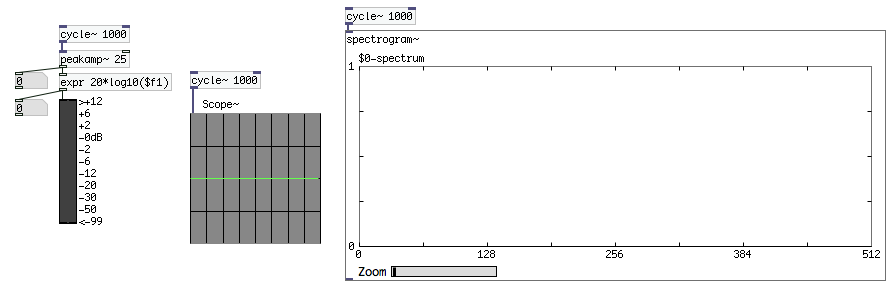
\includegraphics[width = 14cm]{img/metering.png}
		\caption{metering techniques}
		\label{fig:metering}
	\end{center}
\end{figure}




% /*==========  Synth  ==========*/
\section{Synth auffetten}

Was fällt den studenten ein was man machen könnte um den synth fetter zu machen?\\
zB: Polyphonie, unison, Chorus, hall.

\subsection{Polyphonie} % (fold)
\label{sub:polyphonie}

Simplen poly synth from scratch.

\begin{figure}[!h]
	\begin{center}
		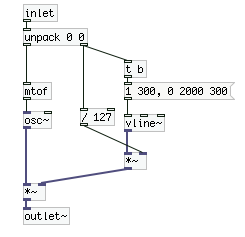
\includegraphics[width = 11cm]{img/SynthVoice1.png}
		\caption{Simple Synth Voice, SynthVoice.pd}
		\label{fig:synthVoice1}
	\end{center}
\end{figure}

\begin{figure}[!htbp]
	\begin{center}
		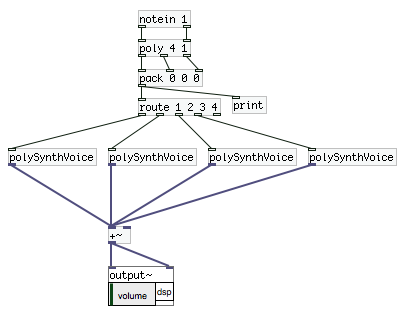
\includegraphics[width = 12cm]{img/PolyHost.png}
		\caption{Example Poly Host, patch 01\_polySynthHost.pd}
		\label{fig:polyHost}
	\end{center}
\end{figure}


\section{Unison}
Supersaw
\section{Hall}
gemeinsam Schroeder paper anschauen. Nachbauen.

\section{Sequencer}
Sequencer + drumpad = wir sparen uns zeit und geld.
\section{drumpad/evenlope following}
Vor der übung buffersize raufstellen!

HUE: eventuell sequence bauen.
